%\documentclass[border=10pt]{standalone}
%\usepackage{tikz}
\tikzset{
	treenode/.style = {shape=rectangle, rounded corners,
		draw, align=center,
		top color=white, bottom color=blue!20},
	root/.style     = {treenode, font=\ttfamily\normalsize, bottom color=red!30},
	env/.style      = {treenode, font=\ttfamily\normalsize},
	dummy/.style    = {circle,draw},
	level 1/.style={sibling distance=6cm, level distance = 3em, label = 1pt },
	level 2/.style={sibling distance=2.3cm,level distance = 5em}, 
	level 3/.style={sibling distance=2cm},
	blueRed/.style={env, top color=blue, bottom color=red} 
}
%\begin{document}
	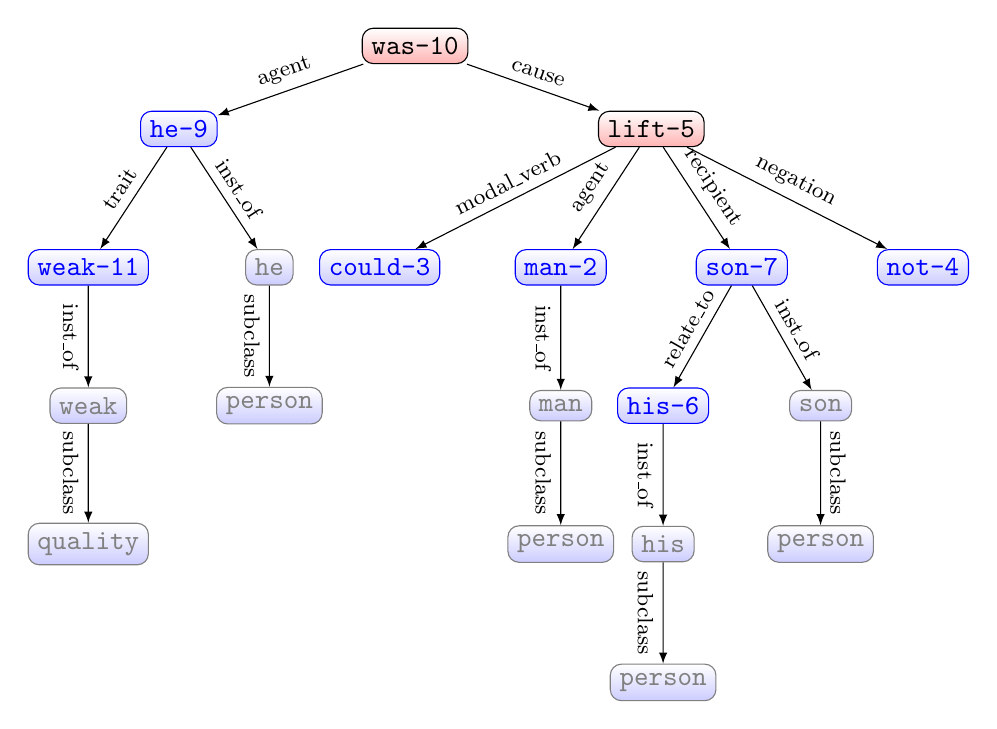
\begin{tikzpicture}
	[
	grow                    = down,
	sibling distance        = 50em,
	level distance          = 5em,
	edge from parent/.style = {draw, -latex},
	every node/.style       = {font=\footnotesize},
	sloped
	]
	\node [root] {was-10}
	child { node [env, blue] {he-9}
	  child {node [env, blue] {weak-11}
	  	 child {node [env, gray] {weak}
	  		child {node [env, gray] {quality}
	  			edge from parent node [below] {subclass}}
	  		edge from parent node [below] {inst\_of}}
			edge from parent node [above] {trait}}
	  child {node [env, gray] {he}
	  		child {node [env, gray] {person}
	  			edge from parent node [below] {subclass}}
	  		edge from parent node [above] {inst\_of}}	
	   edge from parent node [above] {agent}}
	child { node [env, bottom color=red!30] {lift-5} 
	  child {node [env, blue]  {could-3}
	  	edge from parent node [above] {modal\_verb} }	
	  child {node [env, blue]  {man-2}
	  	child {node [env, gray] {man}
	  		 child {node [env, gray] {person}
	  			edge from parent node [below] {subclass}}
	  		edge from parent node [below] {inst\_of}}
	  	edge from parent node [above] {agent} }
	  child {node [env, blue]  {son-7}
	  	child {node [env, blue] {his-6}
	  		child {node [env, gray] {his}
 			  	child {node [env, gray] {person}
  				   edge from parent node [below] {subclass}}
	  			edge from parent node [below] {inst\_of}}
	  		edge from parent node [above] {relate\_to}}
  		child {node [env, gray] {son}
  			child {node [env, gray] {person}
  				edge from parent node [above] {subclass}}
  		 edge from parent node [above] {inst\_of}}
	  	edge from parent node [above] {recipient}}
	  child {node [env, blue]  {not-4}
			edge from parent node [above] {negation} }
		edge from parent node [above] {cause}};
	

	\end{tikzpicture}
%\end{document}